\chapter{Manifolds}

Roughly speaking, a ``manifold'' is a locally flat geometric object without pre-ordained local coordinate systems. Before we formalize what we mean by this, it's useful to philosophize a bit. First of all, let's think about what ``locally flat'' means. Consider, for example, the surface of the earth. On the one hand, we know that it's a sphere (approximately, at least). On the other hand, we also know from personal experience that the curvature of the earth is irrelevant in situations where everything of concern is within a few miles of us. The earth looks flat. It is in this sense that the surface of the earth is ``locally flat.'' 

When we have such a locally flat geometric object, it's often useful to introduce ``local coordinate systems.'' For example, we talk about things being ``in front of'' us or being ``behind'' us in our everyday lives, despite the fact that, if you go far enough forward, you'll eventually end up behind where you started! In other words, ``in front of'' and ``behind'' make no sense if we're thinking globally (ie, if we're thinking at the level of the entirety of the earth). They only make sense ``locally,'' but despite that, they're incredibly useful notions in everyday life. Similar considerations apply with ``left'' and ``right.''

It's also useful to allow local coordinate systems to change depending on the situation we're in. Returning to the example of ``in front of'' and ``behind,'' notice that these notions don't refer to absolute directions: if you turn 90$^\circ$ in some direction, what was ``in front of'' you before you turned isn't ``in front of'' you anymore. After your $90^\circ$ turn, there's now a new useful notion of ``in front of.'' In other words, changing the situation you're in has made a different local coordinate system useful.

Let's now return to the sentence we started with, that ``manifolds are locally flat geometric objects without pre-ordained local coordinate systems.'' We'll see below how to formalize ``locally flat'' mathematically. The way we'll avoid having pre-ordained local coordinate systems is by remembering \emph{all possible choices} of local coordinate systems! 

It's also worth remarking that this chapter marks a somewhat significant turning point in our meditation of derivatives and tangents. We began \cref{single} with the observation that we could formalize our intuitive idea of ``tangent line'' using  derivatives. In the next chapter, we'll see that, in the abstract setting of manifolds, we can formalize the idea of ``tangent vector,'' and then use it to define an even further generalization of the derivative. 

\section{Definition of a manifold}

At this point, we will need to use the language of topological spaces. If you've seen metric spaces but not topological spaces, you should skim through \cref{topological-spaces-basics} (in particular, at least \cref{topological-space-definition,metric-to-topological,continuous-definition,open-map-definition,homeomorphism-definition}).

\subsection{Charts}

Throughout this section, let $X$ be a topological space.\index{topological space} Recall that we want for $X$ to be ``locally flat.'' Formally, this means that we can cover $X$ with open subsets, each of which is ``flat'' in the sense that it is homeomorphic to an open subset of $\R^n$. Notice that, if we remember not just the fact that each open subset $U$ in that cover is homeomorph\emph{ic} to $\R^n$, but the actual homeomorph\emph{ism}, then we can transfer the usual coordinate system on $\R^n$ through the homeomorphism onto $U$. In other words, a homeomorphism between $U$ and an open subset of $\R^n$ tells us both that $U$ is ``flat,'' and gives us a coordinate system on $U$. This is precisely what's accomplished by the following definition. 

\begin{definition}[Chart] \index{chart}
	A \emph{chart} on $X$ is a pair $(U, \phi)$ consisting of an open subset $U \subseteq X$ and a continuous, open\index{open!open map}, and injective function $\phi : U \to \R^n$ for some $n$. 
	\begin{itemize}
		\item The integer $n$ is called the \emph{dimension} of the chart, and write $\dim (U,\phi)$ to denote it. 
		\item The function $x$ is called the \emph{coordinate function} of the chart. 
		\item If $a \in X$, we say that the chart $(U,\phi)$ \emph{contains} $a$ if $a \in U$. If $(U,\phi)$ contains $a$ and $\phi(a) = 0$, we say that $(U,\phi)$ is \emph{centered at} $a$. 
		\item For all $i = 1, \dotsc, n$, we define $\phi_i := \pi_i \circ \phi$. For any $a \in U$, the real numbers $\phi_1(a), \dotsc, \phi_n(a)$ are called the \emph{coordinates of $a$ with respect to the chart  $(U,\phi)$}.\index{coordinates}
	\end{itemize} 
\end{definition}

\begin{example} \label{polar-representation}
	Let $X = \R^2$ and let $U$ denote $\R^2$ minus the non-negative $x$-axis. In other words, 
	\[ U = \{(x,y) : x < 0 \text{ or } y \neq 0 \}. \]
	Let $\phi : U \to \R^2$ be the function which sends a point $p$ to its polar representation $\phi(p) = (r(p), \theta(p))$, where $r(p) = |p|$ and $\theta(p)$ is the angle in radians strictly between 0 and $2\pi$ formed between $p$ and the non-negative real axis. Let us show that $(U, \phi)$ is a chart. 
	
	Observe that $\phi$ is injective, we have
	\[ \phi(U) = \{ (r, \theta) : r > 0, \theta \in (0, 2\pi) \}, \]
	and the inverse function of $\phi$ is given by  $\phi^{-1}(r,\theta) = (r\cos \theta, r\sin\theta)$. Clearly $\phi^{-1}$ is continuous. In fact, it is even \'etale, since 
	\[ \det (\phi^{-1})'(r, \theta) = \det \begin{bmatrix} \cos \theta & -r\sin\theta \\ \sin\theta & r\cos \theta \end{bmatrix} = r^2 \neq 0 \]
	on $\phi(U)$, so the inverse function theorem \ref{inverse-function-theorem} tells us that $\phi^{-1}$ is open. This means that $\phi$ is continuous as well, proving that $(U, \phi)$ is a chart. 
	
	Notice that the chart $(U, \phi)$ contains the point $(1,1)$. We calculate the coordinates of $(1,1)$ with respect to this chart by evaluating $\phi(1,1)$. We find
	\[ \rho(1,1) = (\sqrt{1^2 + 1^2}, \arctan(1)) = (\sqrt{2}, \pi/4). \]
	In other words, $\phi$ outputs precisely the polar representation of $(1,1)$. 
\end{example}

\begin{remark} \label{recentering-chart}
	If $(U,\phi)$ is a chart on $X$ and $a \in U$  is a point, we can ``recenter the chart at $a$'' by replacing $\phi$ with the function $\tilde{\phi}$ given by $\tilde{\phi}(x) = \phi(x) - \phi(a)$. In other words, if $\tilde{\phi} = \phi - \phi(a)$, then $(U, \tilde{\phi})$ is also a chart, and we have $\tilde{\phi}(a) = 0$.
\end{remark}

\subsection{Compatibility of charts}

Charts formalize the idea of local coordinate systems; the following formalizes the idea of \emph{changing} local coordinate systems. 

\begin{definition}[Transition function] \label{transition-map} \index{transition function}
	Suppose $(U, \phi)$ and $(V, \psi)$ are charts on $X$. The \emph{transition function} from $(U, \phi)$ to $(V, \psi)$ is the function $\psi \circ \phi^{-1}$.
	\[ \begin{tikzcd}
	\phi(U \cap V) \ar{r}{\phi^{-1}} & U \cap V \ar{r}{\psi} & \psi(U \cap V)
	\end{tikzcd} \]
	Notice that the domain $\phi(U \cap V)$ is an open subset of $\R^m$ for $m = \dim(U, \phi)$ and the codomain $\psi(U \cap V)$ is an open subset of $\R^n$ for $n = \dim(V, \psi)$. In other words, $\psi \circ \phi^{-1}$ is precisely the kind of function whose derivative we studied in \cref{multi}. 
\end{definition}

\begin{definition}[Compatibility of charts] \index{compatibile} \label{compatibility}
	The two charts $(U, \phi)$ and $(V, \psi)$ on $X$ are \emph{smoothly compatible}, or just \emph{compatible}, if the transition map $\psi \circ \phi^{-1}$ from $(U, \phi)$ to $(V, \psi)$ and the transition map $\phi \circ \psi^{-1}$ from $(V, \psi)$ to $(U, \phi)$ are smooth. 
\end{definition}

\begin{example} \label{cube-not-compatible}
	Let $\id : \R \to \R$ denote the identity map and let $\phi : \R \to  \R$ denote the map $\phi(x) = x^3$. Both maps are homeomorphisms, so $(\R, \id)$ and $(\R, \phi)$ are charts. However, these two charts are not compatible. The transition function from $(\R, \id)$ to $(\R, \phi)$ is 
	\[ \begin{tikzcd} \R = \id(\R) \ar{r}{\id^{-1}} & \R \ar{r}{\phi} & \phi(\R) = \R, \end{tikzcd} \]
	which is just $\phi$, which is in fact smooth. However, in the other direction, the transition function is 
	\[ \begin{tikzcd} \R = \phi(\R) \ar{r}{\phi^{-1}} & \R \ar{r}{\phi} & \id(\R) = \R, \end{tikzcd} \]
	which is the function $\phi^{-1}(x) = \sqrt[3]{x}$. In other words, the transition function from $(\R, \phi)$ to $(\R, \id)$ is not even differentiable. 
\end{example}

\begin{exercise}
	Determine whether or not each of the following charts $(U, \phi)$ is compatible with $(\R, \id)$.
	\begin{enumerate}[(a)]
		\item $U = \R$ and $\phi(x) = 2x$.
		\item $U = \R$ and $\phi(x) = -x$. 
		\item $U = \R$ and $\phi(x) = x|x|$. 
		\item $U = \R$ and $\phi(x) = -x^3$. 
		\item $U = (-\pi/2, \pi/2)$ and $\phi(x) = \tan(x)$. 
		\item $U = (0, \infty)$ and $\phi(x) = \ln(x)$. 
		\item $U = \R$ and $\phi(x) = x^5$. 
	\end{enumerate}
	Use these examples to formulate a conjecture for determining when a chart $(U, \phi)$ on $\R$ is compatible with $(\R, \id)$. Then prove your conjecture. 
\end{exercise}

\begin{example} \label{polar-compatible-with-identity}
	Let $\id : \R^2 \to \R^2$ denote the identity map and $\phi : U \to \R^2$ the polar representation map from \cref{polar-representation}. The two charts $(\R^2, \id)$ and $(U, \rho)$ are compatible. To see this, observe that the transition function from $(U, \phi)$ to $(\R^2, \id)$ is the function
	\[ \begin{tikzcd} \phi(U) \ar{r}{\phi^{-1}} & U \ar{r}{\id} & \id(U) = U, \end{tikzcd} \]
	which is just $\phi^{-1}$. We saw in \cref{polar-representation} that $\phi^{-1}$ is given explicitly by \[ \phi^{-1}(r, \theta) = (r\cos\theta, r\sin\theta), \]
	which is a smooth function. Going the other way, the transition function from $(\R^2, \id)$ to $(U, \phi)$ is precisely $\phi$. 
	\[ \begin{tikzcd} U = \id(U) \ar{r}{\id^{-1}} \ar{r} & U \ar{r}{\phi} & \phi(U) \end{tikzcd} \]
	As we saw in \cref{polar-representation}, the map $\phi^{-1}$ is \'etale, so its inverse function $\phi$ is smooth by \cref{ck-stable-inversion}. Thus both transition functions are smooth, so the two charts are compatible. 
\end{example}

\begin{exercise}
	Show that two charts $(U,\phi)$ and $(V, \psi)$ are compatible if and only if the transition function from $(U, \phi)$ to $(V,\psi)$ is smooth and \'etale. 
\end{exercise}

\begin{exercise}
	Suppose $(U, \phi)$ is a chart and $a \in X$ is a point. Consider the recentered chart $(U, \tilde{\phi})$ where $\tilde{\phi} = \phi - \phi(a)$, as in \cref{recentering-chart}. Show that $(U, \phi)$ and $(U, \tilde{\phi})$ are compatible. 
\end{exercise}

\begin{remark} \label{compatibility-not-equivalence-relation}
	An important cautionary observation is that compatibility of charts is \emph{not} an equivalence relation on the set of all charts. It is certainly reflexive and symmetric, but it fails to be transitive. For example, let $\phi(x) = x^3$ and then consider the three charts $(\R, \id), (\R \setminus \{0\}, \phi)$, and $(\R, \phi)$. The first two are compatible with each other, and the second two are compatible with each other, but the first and third are \emph{not} compatible with each other (cf.  \cref{cube-not-compatible}). 
\end{remark}

\begin{exercise} \label{dimension-well-defined}
	Suppose $(U, \phi)$ and $(V, \psi)$ are compatible charts and that the intersection $U \cap V$ is nonempty. Show that $\dim(U,\phi) = \dim(V,\psi)$. 
	\begin{hint}
		Fix a point $a \in U \cap V$, and consider the derivative of the transition function $\psi \circ \phi^{-1}$ at $\phi(a)$. 
	\end{hint}
\end{exercise}

\subsection{Atlases and manifolds}

\begin{definition}[Atlas] \index{atlas} \index{atlas!maximal atlas} \index{maximal atlas|see {atlas, maximal atlas}}
	An \emph{atlas} on $X$ is a collection $\mathscr{A}$ of compatible charts such that covers $X$. In other words, a collection $\mathscr{A}$ of charts is an atlas if every pair of charts in $\mathscr{A}$ is compatible, and \[ \bigcup_{(U, \phi) \in \mathscr{A}} U = X. \]
	If $\mathscr{A}'$ is also an atlas and $\mathscr{A}' \subseteq \mathscr{A}$, we say that $\mathscr{A}'$ is a \emph{sub-atlas} of $\mathscr{A}$. An atlas is \emph{maximal} if there is no strictly larger atlas containing it.
\end{definition}

\begin{exercise}[Existence and uniqueness of maximal atlases] \label{existence-maximal-atlas}
	Prove that every atlas $\mathscr{A}$ is contained in a unique maximal atlas.\index{atlas!maximal atlas} 
	\begin{hint}
		Let $\mathscr{A}'$ be the set of all charts that are compatible with all of the charts in $\mathscr{A}$. Prove that $\mathscr{A}'$ is an atlas (caution: keep \cref{compatibility-not-equivalence-relation} in mind). Then prove that it is maximal, and that it is the only maximal atlas containing $\mathscr{A}$. 
	\end{hint}
\end{exercise}

\begin{exercise}
	Suppose $\mathscr{A}$ and $\mathscr{A}'$ are two atlases on $X$. Let us say that $\mathscr{A}$ and $\mathscr{A}'$ are \emph{compatible} if the union $\mathscr{A} \cup \mathscr{A}'$ is an atlas. 
	\begin{enumerate}[(a)]
		\item  Show that the following are equivalent. 
		\begin{enumerate}[(i)]
			\item $\mathscr{A}$ and $\mathscr{A}'$ are compatible. 
			\item Each chart in $\mathscr{A}$ is compatible with every chart in $\mathscr{A}'$. 
			\item $\mathscr{A}$ is a sub-atlas of the unique maximal atlas that contains $\mathscr{A}'$. 
		\end{enumerate}
		\item Show that compatibility \emph{is} an equivalence relation on the set of all atlases on $X$.
	\end{enumerate} 
	Make sure you understand how the assertion made in part (b) above differs from the assertion in \cref{compatibility-not-equivalence-relation}. Compatibility of  \emph{charts} is not an equivalence relation, compatibility of \emph{atlases} is. 
\end{exercise}

This leads us to the following definition.

\begin{definition}[Manifold] \index{manifold} \index{smooth manifold|see {manifold}}
	A \emph{smooth manifold}, or just a \emph{manifold}, is a pair $(X, \mathscr{A}_X)$ where $X$ is a topological space and $\mathscr{A}_X$ is a maximal atlas. Often, we just write ``$X$'' in place of the pair $(X, \mathscr{A}_X)$. Sometimes the maximal atlas $\mathscr{A}_X$ is called the \emph{manifold structure} or the \emph{smooth structure} on $X$.
\end{definition}

\Cref{existence-maximal-atlas} tells us that any not-necessarily-maximal atlas on a topological space $X$ can be extended uniquely to a maximal atlas, thus giving $X$ the structure of a manifold. When constructing examples, we will usually give an explicit finite non-maximal atlas and then use \cref{existence-maximal-atlas} to extend it to a maximal atlas; it is difficult to describe maximal atlases explicitly, because there are many, many charts in maximal atlases. But it is often convenient for theorem statements and abstract proofs to assume that the atlas that the manifold comes equipped with is already maximal, which is why the definition is made the way it is.

\begin{unimportantremark}
	For any $k = 0, 1, 2, \dotsc, \infty$, we could define charts to be \emph{$C^k$-compatible} by requiring that the transition functions between them are $C^k$ (rather than smooth, as in \cref{compatibility}). This would lead to a definition of \emph{$C^k$-manifolds}. In these notes, we'll just stick to the $k = \infty$ case.  
\end{unimportantremark}

\subsection{Dimension}

\begin{definition}[Dimension] \index{dimension!of a manifold}
	Suppose $X$ is a manifold and $a \in X$ is a point. By \cref{dimension-well-defined}, there is a unique integer $n$ such that $\dim(U,\phi) = n$ for every chart $(U, \phi) \in \mathscr{A}_X$ containing $a$. This integer is called the \emph{dimension of $X$ at $a$}, and is denoted $\dim_a(X)$. If there exists a single integer $n$ such that $\dim_x(X) = n$ for all $x \in X$, we say that $X$ is \emph{equidimensional} and that the \emph{dimension of $X$} is $n$. 
\end{definition}

\begin{proposition}
	If the set $\N$ of natural numbers is given the discrete topology, the function $X \to \N$ given by $x \mapsto \dim_x(X)$ is continuous. In particular, if $X$ is a nonempty connected manifold, it must be equidimensional. 
\end{proposition}

\begin{proof}
	To show that $x \mapsto \dim_x(X)$ is continuous, we want to show that, for any natural number $n$, the set 
	\[ X_n = \{ x \in X : \dim_x(X) = n \} \]
	is an open subset of $X$. Suppose $a \in  X_n$. Let $(U, \phi)$ be a chart containing $a$. Then $\dim(U,\phi) = n$, and we have $\dim_x(X) = n$ for all $x \in U$. In other words, $U \subseteq X_n$. Thus, for every $a \in X_n$, there exists an open neighborhood of $a$ that is entirely contained inside $X_n$, so $X_n$ is open. 
	
	Now suppose $X$ is connected and $a \in X$. Let $n = \dim_a(X)$, so that $a \in X_n$. Then 
	\[ X \setminus X_n = \bigcup_{m \neq n} X_m \]
	is a union of open sets and is therefore also open. Thus $X_n$ is a nonempty subset of $X$ that is both open and closed. Since $X$ is connected, we conclude that $X = X_n$. In other words, $X$ is equidimensional of dimension $n$. 
\end{proof}

\section{Examples}

\subsection{First examples}

\subsubsection*{Euclidean space}

\begin{example} \label{natural-euclidean-atlas}
	The single chart $(\R^n, \id)$, where $\id : \R^n \to \R^n$ is the identity map, defines an atlas on $\R^n$. We can extend this to a maximal atlas, called the \emph{euclidean atlas} on $\R^n$. Unless explicitly specified otherwise, we always regard $\R^n$ as a manifold by equipping it with the euclidean atlas. The polar representation chart of  \cref{polar-representation,polar-compatible-with-identity} is an element of the euclidean atlas on $\R^2$. 
\end{example}

\begin{exercise}
	For any $r > 0$, let $\phi_r : \R \to \R$ be the function
	\[ \phi_r(t) = \begin{cases} t & \text{if } t \leq 0 \\ rt & \text{if } t > 0. \end{cases} \]
	Note that $\phi_r$ is continuous and strictly increasing (hence also injective and open, by \cref{strictly-monotone-iff-injective,strictly-monotone-implies-open}), so $(\R, \phi_r)$ is a chart. Note also that $\phi_1 = \id$. 
	\begin{enumerate}[(a)]
		\item Show that $\phi_s \circ \phi_r = \phi_{sr}$ and that $(\phi_r)^{-1} = \phi_{1/r}$. 
		\item Show that $(\R, \phi_r)$ and $(\R, \phi_s)$ are compatible if and only if $r = s$.
		\item Let $\mathscr{A}_r$ be the maximal atlas obtained by extending $(\R, \phi_r)$. What can you say about $\mathscr{A}_r$ and $\mathscr{A}_s$ if $r \neq s$? Are any of these the euclidean atlas? What can you conclude about the number of maximal atlases on $\R$?
	\end{enumerate}  
\end{exercise}

\begin{exercise} \label{euclidean-chart-characterization}
	Suppose $U$ is an open subset of $\R^n$ and $\phi : U \to \R^n$ is a function. Show that the pair $(U, \phi)$ is a chart in the euclidean atlas on $\R^n$ if and only if $\phi$ is injective, smooth, and \'etale.
\end{exercise}

\subsubsection*{Circles and spheres}

\begin{exercise}[The circle $S^1$] \index{s1@$S^1$|see {circle}} \index{circle} \label{circle-projection-atlas}
	Let $S^1$ denote the set of points in $\R^2$ along the unit circle. In other words,
	\[ S^1 = \{ (x, y) \in \R^2 : x^2 + y^2 = 1 \}. \]
	\begin{enumerate}[(a)]
		\item Do \cref{metric-subspace}. This shows that both ways that we might think to regard $S^1$ as a topological space are actually the same. 
		
		\item Let $U = S^1 \setminus \{(0,1)\}$. For a point $a \in S^1$, let $\phi(a)$ denote the $x$-coordinate of the point where the line $y = -1$ intersects the line passing through $(0,1)$ and $a$. This is sometimes called ``projection from the north pole.'' See \cref{circle-projection}. If $a = (x,y)$, find an explicit formula for $\phi(a)$ in terms of $x$ and $y$. 
		
		\begin{figure}
			\begin{center}
				\begin{tikzpicture}
				\begin{axis}[
				xmin=-1.5,xmax=1.5,
				ymin=-1.3,ymax=1.3,
				ytick={-1,1},
				xtick={-1,1},
				xticklabels={},
				yticklabels={},
				axis lines=middle,
				axis line style=lightgray,
				width=\textwidth,
				axis equal
				]
				
				\addplot[black,style=thick,-] expression[domain=-1:1,samples=200]{sqrt(1-x^2)}; 
				\addplot[black,style=thick,-] expression[domain=-1:1,samples=200]{-sqrt(1-x^2)};
				
				
				\addplot[red,<->] expression[domain=-0.1:0.95,samples=2]{-2.414*x+1}; 
				
				
				\addplot[black,<->] expression[domain=-1.5:1.5,samples=2]{-1};
				
				\node[label={85:{$(0,1)$}},color=white,draw=black,circle,fill,inner sep=2pt] at (axis cs:0,1) {}; 
				\node[label={0:{$a$}},color=black,draw=black,circle,fill,inner sep=2pt] at (axis cs:0.707,-0.707) {}; 
				\node[color=red,draw=red,circle,fill,inner sep=2pt] at (axis cs:0.8285,-1) {}; 
				
				\end{axis}
				\end{tikzpicture}
			\end{center}
			\caption{Given a point $a \in U = S^1 \setminus \{(0,1)\}$, we draw a line connecting $a$ to $(0,1)$, indicated in red. The point where that line intersects the line $y = -1$ (in black) is sometimes called the ``projection'' of $a$ from $(0,1)$ onto $\R \times \{-1\}$. The $x$-coordinate of this point is $\phi(a)$.}  \label{circle-projection}
		\end{figure}
		
		\item Show that $\phi : U \to \R$ is a homeomorphism.\index{homeomorphism} Thus $(U, \phi)$ is a chart on $S^1$. 
		\begin{hint} 
			Use geometry to write down a formula for the inverse function to $\phi$. 
		\end{hint}
		
		\item Let $V = S^1 \setminus \{(0,-1)\}$. For $a \in V$, let $\psi(a)$ denote the $x$-coordinate of the point where the line $y = 1$ intersects the line passing through $(0,-1)$ and $a$. Show that $\psi : V \to \R$ is also a homeomorphism. 
		
		\item Show that $(U, \phi)$ and $(V, \psi)$ are compatible charts. Thus $\mathscr{A} = \{(U, \phi), (V, \psi)\}$ is an atlas on $S^1$. Extending $\mathscr{A}$ to a maximal atlas $\mathscr{A}_{S^1}$, we have defined a manifold structure on $S^1$.
		
		\item Let $W = \{ (x,y) \in S^1 : x > 0 \}$ be the ``right half of the circle.'' If $\pi : W \to \R$ is the function $\pi(x,y) = y$, show that $(W,\pi)$ is a chart and that it is compatible with the two charts in the atlas $\mathscr{A}$ constructed above. Thus $(W, \pi) \in \mathscr{A}_{S^1}$. 
		
		\item Can you think of any other charts in the maximal atlas $\mathscr{A}_{S^1}$, besides the three discussed above?
		
		\begin{hint}
			There are many, many possibilities here. You could project other halves of the circle onto the $x$-axis or the $y$-axis, like in (f). More interestingly, you could also think about charts defined using trigonometric functions. 
		\end{hint}
	\end{enumerate}
\end{exercise}

\begin{exercise}[The $n$-sphere $S^n$] \label{sphere-projection-atlas} \index{sn@$S^n$|see {$n$-sphere}} \index{n-sphere@$n$-sphere}
	Let $S^n$ denote the set of points in $\R^{n+1}$ that have euclidean norm 1. Generalize \cref{circle-projection-atlas} and show that ``projection from the north pole'' and ``projection from the south pole'' define an atlas on $S^n$. 
\end{exercise}

\subsubsection*{Matrices and vector spaces}

\begin{example}[Matrices]
	There is an isomorphism of vector spaces $\phi : \mathscr{M}_{n \times m} \to \R^{mn}$\index{mnm@$\mathscr{M}_{n \times m}$} where, if $A \in \mathscr{M}_{n \times m}$ has entries $a_{i,j}$, then
	\[ \phi(A) = \begin{bmatrix} a_{1,1} \\ a_{1,2} \\ \vdots \\ a_{1,m} \\ a_{2,1} \\ \vdots \\ a_{n,m} \end{bmatrix}. \]
	If we endow $\mathscr{M}_{n \times m}$ with the canonical topology,\index{canonical topology} then $\phi$ is automatically a homeomorphism by \cref{linear-isomorphism-homeomorphism}.\index{homeomorphism} In other words, the single chart $(\mathscr{M}_{n \times m}, \phi)$ is an atlas on $\mathscr{M}_{n \times m}$. Extending it to a maximal atlas using \cref{existence-maximal-atlas}, we see that we can regard $\mathscr{M}_{n,m}$ as a manifold. It is $mn$-dimensional.  
\end{example}

The same process discussed above allows us to regard \emph{any} finite dimensional vector space as a manifold. 

\subsubsection*{Constructions}

\begin{exercise}[Graphs of continuous functions] \label{graphs-continuous}
	Suppose $U$ is an open subset of $\R^m$ and $f : U \to \R^n$ is a continuous function. 
	\begin{enumerate}[(a)]
		\item There are two ways we might think to regard $U \times \R^n$ as a topological space. One way is to use the product topology \ref{product-space}. The second way is to regard $U \times \R^n$ as a subset of $\R^m \times \R^n = \R^{m+n}$ and then give $U \times \R^n$ the subspace topology \ref{subspace-topology}. Show that these two topologies are the same. 
		
		\item Let $\Gamma = \{ (x,y) \in U \times \R^n : f(x) = y \}$ be the graph of $f$, regarded as a subspace of $U \times \R^n$. Show that the function $\pi : \Gamma \to \R^m$ given by $\pi(x,y) = x$ is continuous, injective, and open. 
	\end{enumerate}
	Thus the single chart $(\Gamma, \pi)$ defines an atlas on $\Gamma$. Extending this to a maximal atlas, we can regard $\Gamma$ as a manifold. 
\end{exercise}

\begin{exercise}[Open submanifolds] \label{open-submanifold}
	Let $X$ be a manifold and $U \subseteq X$ an open subset. Show that \[ \mathscr{A}_U = \{ (V,\phi) \in \mathscr{A}_X : V \subseteq U \} \]
	is a maximal atlas on $U$. We call $U$, equipped with this maximal atlas, an \emph{open submanifold} of $X$. 
\end{exercise}

\begin{exercise}[Product manifold]
	Let $X$ and $Y$ be manifolds. Let $\mathscr{A}$ be the set of charts of the form $(U \times V, \phi \times \psi)$, where $(U, \phi) \in \mathscr{A}_X$, $(V, \psi) \in \mathscr{A}_Y$, and $\phi \times \psi$ denotes the natural map $U \times V \to \R^m \times \R^n = \R^{m+n}$, where $m = \dim(U,\phi)$ and $n = \dim(V, \psi)$. Show that $\mathscr{A}$ is an atlas on $X \times Y$. We call $X \times Y$, equipped with the corresponding maximal atlas, the \emph{product manifold}. 
\end{exercise}

\subsection{M\"obius strip}

Let $B$ denote the box $[0,1] \times (0,1)$ inside $\R^2$, and let $\sim$ be the equivalence relation on $B$ generated by declaring $(0,y) \sim (1,1-y)$ for all $y \in (0,1)$. 
See \cref{mobius-box}. The equivalence class of a point $(x,y) \in B$ is denoted by $[x,y]$. Observe that every equivalence class contains either 1 or 2 elements. The \emph{M\"obius strip}\index{mobius strip@M\"obius strip} $M$ is the set of equivalence classes in $B$. In other words, we take the box $[0,1] \times (0,1)$ and ``glue'' its left and right edges, with a twist. If you've ever made a M\"obius strip out of paper, you can probably see that we've formalized exactly that same process. See \cref{mobius-box}, again.

\begin{figure}
	\begin{center}
	\begin{tikzpicture}
	\begin{axis}[
	xmin=-0.1,xmax=1.1,
	ymin=-0.1,ymax=1.1,
	ytick={1},
	xtick={1},
	xticklabels={1},
	yticklabels={1},
	axis lines=middle,
	axis line style=lightgray,
	axis equal,
	width=0.6\textwidth
	]
	
	\addplot[black, opacity=0.2, domain=0:1, samples=2] {0.25};
	\addplot[black, opacity=0.2, domain=0:1, samples=2] {0.75};
	
	\foreach \n in {1, ..., 9}
		\addplot +[mark=none, black, solid, opacity=0.2] coordinates {(0.1*\n, 0) (0.1*\n, 1)};
	
	\addplot[black, dashed, name path=top, domain=0:1, samples=2] {0};
	\addplot[black, dashed, name path=bottom, domain=0:1, samples=2] {1};
	\addplot [fill=red, fill opacity=0.1] 
	fill between[of=top and bottom];
	
	
	\addplot[red, thick, domain=0:1, samples=2, opacity=0.5] {0.5};
	\addplot +[mark=none, solid, thick, black] coordinates {(0, 0) (0, 1)};
	\addplot +[mark=none, solid, thick, black] coordinates {(1, 0) (1, 1)};
	
	\node[color=black,draw=black,circle,fill,inner sep=2pt] at (axis cs:0,0.25) {}; 
	\node[color=black,draw=black,circle,fill,inner sep=2pt] at (axis cs:1,0.75) {}; 
	\end{axis}
	\end{tikzpicture}
	
	\vspace{2em}
	
	
	\caption{Above is a picture of the box $B = [0,1] \times (0,1)$ and the equivalence relation $\sim$ described above. Geometrically, this equivalence relation identifies the vertical black line on the left of the box with the vertical black line on the right of the box, but ``with a twist.'' For example, the point $(0,1/4)$ on the left is identified with the point $(1,3/4)$ on the right. If we pick up the box and actually glue together the edges as indicated by the equivalence relation, we end up with the M\"obius strip as pictured below.} \label{mobius-box}
	
	\vspace{3em}
	
	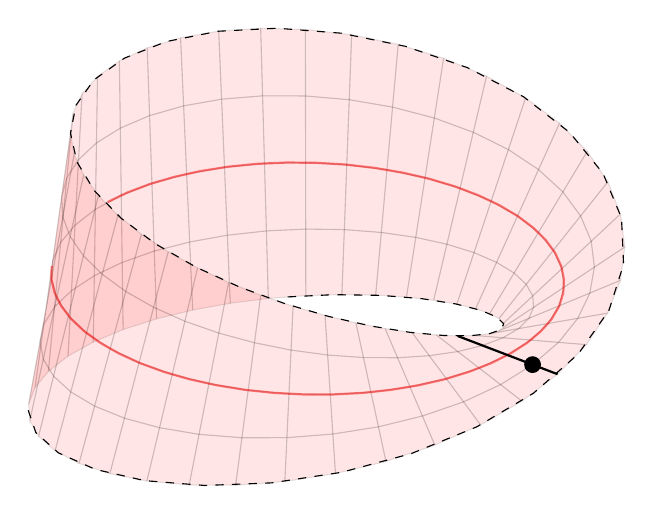
\begin{tikzpicture}
	\begin{axis}[
	hide axis,
	view={40}{40},
	width=\textwidth]
	
	\addplot3 [surf,
	red,
	opacity=0.1,
	faceted color=black,
	point meta=x,
	samples=40,
	samples y=5,
	z buffer=sort,
	domain=0:360,
	y domain=-0.5:0.5
	] (
	{(1+0.5*y*cos(x/2)))*cos(x)},
	{(1+0.5*y*cos(x/2)))*sin(x)},
	{0.5*y*sin(x/2)});
	
	% Center line
	\addplot3 [samples=50, domain=-145:180, samples y=0, red, thick, opacity=0.5
	] ({cos(x)},{sin(x)},{0});
	
	% Outside line
	\addplot3 [samples=50, domain=-135:495, samples y=0, black, dashed] (
	{(1+0.25*cos(x/2)))*cos(x)},
	{(1+0.25*cos(x/2)))*sin(x)},
	{0.25*sin(x/2)});
	
	% Glued line
	\addplot3 [samples=50,domain=-0.5:0.5,samples y=0, black, thick,
	] ({1+0.5*x},{0},{0});
	
	% Point
	\node[color=black,draw=black,circle,fill,inner sep=2pt] at (axis cs:1+1/8,0,0) {};
	\end{axis}
	\end{tikzpicture}
	\end{center}
\end{figure}

We regard $M$ as a topological space using the quotient topology, as in \cref{quotient-space}. To give $X$ the structure of a manifold, we will construct an atlas consisting of two charts. But, before proceeding with the formalism, let's describe the intuition. Imagine making a cut in the M\"obius strip corresponding to a vertical cut in the box $B$ (ie, a cut perpendicular to the central red circle in \cref{mobius-box}). Once we make such a cut, we can untwist the M\"obius strip and we're left with an open rectangle, which we can regard as an open subset of $\R^2$. In other words, we've defined a chart on $M$. The points along the cut are missing from this chart; but if we construct a second chart by making a second separate cut, we will have constructed two charts that cover $M$. 

Let's formalize this now. The easiest place to cut is the line along which we glued the M\"obius strip in the first place. In other words, we let \[ U = \{ [x, y] \in M : x \in (0,1) \} \] 
and let $\phi : U \to \R^2$ be the function $\phi([x,y]) = (x, y)$.

\begin{exercise} \label{first-chart-mobius}
	Show that $U$ is an open subset of $M$, and that the function $\phi : U \to \R^2$ is well-defined, continuous, injective, and open. 
\end{exercise}

\begin{solution}{\cref{first-chart-mobius}}
	Let $\pi : B \to M$ be the map $\pi(x,y) = [x,y]$. To show that $U = \{[x,y] \in M : x \neq 0,1\}$ is open, we use the definition of the quotient topology \cref{quotient-space}, which tells us that $U$ is an open subset of $M$ precisely when $\pi^{-1}(U)$ is an open subset of $B$. But \[ \pi^{-1}(U) = B^\circ = (0,1) \times (0,1) \] is an open subset of $B$, so $U$ is open in $M$. 
	
	The facts that $\phi : U \to \R^2$ is well-defined and injective follow immediately from the observation that every equivalence class in $U$ has exactly one element. To see that $\phi$ is continuous, suppose $W$ is an open subset of $\R^2$. We want to show that $\phi^{-1}(W)$ is open in $U$, ie, that $\pi^{-1}(\phi^{-1}(W))$ is open in $B$. But $\pi^{-1}(\phi^{-1}(W)) = B^\circ \cap W$ is an intersection of two open subsets, so it is also open. 
	
	To see that $\phi$ is open, suppose $W$ is an open subset of $U$. We want to show that $\phi(W)$ is an open subset of  $\R^2$. But notice that $\phi(W) = \pi^{-1}(W)$, and we know that $\pi^{-1}(W)$ is open in $B$ by the definition of open subsets in the quotient topology. Moreover, $\phi(W) \subseteq B^\circ$, so $\phi(W)$ is an open subset of $B^\circ$. Since $B^\circ$ is open in $\R^2$, we conclude that $\phi(W)$ is open in $\R^2$. 
\end{solution}

The second chart is a bit harder to describe mathematically, but the intuitive idea is the same. We'll cut the M\"obius strip along the line corresponding the vertical line $x = 1/2$ in $B$. Formally, let \[ V = \{ [x, y] \in M : x \neq 1/2 \} \] and let $\psi : V \to  \R^2$ be the function defined by 
\[ y([x, y]) = \begin{cases} (x, y) & \text{if } x < 1/2 \\ (x-1, 1-x) & \text{if } x > 1/2 \end{cases} \]

\begin{exercise} \label{second-chart-mobius}
	Show that $V$ is also an open subset of $M$, and that $\psi : V \to \R^2$ is well-defined, continuous, injective, and open. 
\end{exercise}

\begin{solution}{\cref{second-chart-mobius}}
	Let $\pi : B \to M$ be the map $\pi(x, y) = [x,y]$ again. Observe that $\pi^{-1}(V) = \{ (x,y) \in B : x \neq 1/2 \}$  is an open subset of $B$ (even though it is not an open subset of $\R^2$), so by definition of the quotient topology, $V$ is an open subset of $M$. 
	
	Let us check that $\psi$ is well-defined. Most equivalence classes have just one element, and $\psi$ is clearly well-defined on those equivalence classes. Equivalence classes with two points are of the form $[0,y] = [1,1-y]$ for some $y \in (0,1)$. Observe that 
	\[ \psi([1,1-y]) = (0,1-(1-y)) = (0,y) = \psi([0,y]), \]
	which shows that $\psi$ is well-defined on the equivalence classes with two elements as well. 
	The verification that $\psi$ is continuous, injective, and open will be left to the reader. 
\end{solution}

\begin{exercise} \label{mobius-charts-compatible}
	Show that $(U, \phi)$ and $(V, \psi)$ are compatible.
\end{exercise}

\begin{solution}{\cref{mobius-charts-compatible}}
	Observe that the transition function $\psi \circ  \phi^{-1}$ from $(U,\phi)$ to $(V,\psi)$ is the composite 
	\[ \begin{tikzcd} \phi(U \cap V) \ar{r}{\phi^{-1}} & U \cap V \ar{r}{\psi} & \psi(U \cap V) \end{tikzcd} \]
	given by 
	\[ (\psi \circ \phi^{-1})(x,y) = \psi([x,y]) = \begin{cases} (x,y) & \text{if } x < 1/2 \\ (x-1, 1-y) & \text{if } x > 1/2 \end{cases} \]
	which is clearly smooth, and 
	\[ (\psi \circ \phi^{-1})'(x,y) = \begin{cases} \begin{bmatrix} 1 & 0 \\ 0 & 1 \end{bmatrix} & \text{if } x < 1/2 \\ \begin{bmatrix} 1 & 0 \\ 0 & -1 \end{bmatrix} & \text{if } x > 1/2 \end{cases} \]
	which shows that $\psi \circ \phi^{-1}$ is \'etale. Thus the two charts are compatible. 
\end{solution}

Thus $\mathscr{A} = \{(U, \phi), (V, \psi)\}$ is an atlas on the M\"obius strip $M$. Letting $\mathscr{A}_M$ denote the corresponding maximal atlas, we obtain the structure of a manifold on $M$.

\begin{exercise}
	Fix a constant $c \in [0,1)$, and let $U_c$ be the subset of $M$ where we've cut out the vertical line $x = c$. Show that $U_c$ is an open subset of $M$. Write down a formula for a well-defined function $\phi_c : U_c \to \R^2$ which is continuous, injective, and open; the image of $\phi_c$ should be an open box in $\R^2$, and you should recover the function $\phi$ above when $c = 0$, and the function $\psi$ when $c = 1/2$. Then show that $(U_c, \phi_c) \in \mathscr{A}_M$ for all $c \in [0,1)$. 
\end{exercise}

\subsection{More quotient examples}

Here are some more examples of manifolds you probably recognize which you probably recognize. 

\begin{exercise}[Cylinder] \label{cylinder}
	Let $S$ denote the infinite vertical strip $[0,1] \times \R$ inside $\R^2$, and let $\sim$ be the equivalence relation generated by $(0,y) \sim (1,y)$ for all $y \in \R$. Let $C$ be the corresponding quotient space. Describe an atlas on $C$. 
\end{exercise}

\begin{exercise}[Torus] \label{torus} \index{torus}
	Let $B$ denote the box $[0,1] \times [0,1]$ inside $\R^2$ and let $\sim$ denote the equivalence relation generated by $(x,0) \sim (x,1)$ and $(0,y) \sim (1,y)$ for all $x,y \in [0,1]$. The \emph{torus} $T$ is defined to be the corresponding quotient space. Describe an atlas on $T$. 
\end{exercise}

% TODO: Torus picture

Sometimes quotient spaces can be very difficult to visualize directly; the only way to have geometric intuition in these cases is to remember the space we started with before quotienting, and the equivalence relation we defined on it. 

\begin{exercise}[Projective line] \label{rp1} \index{projective line} \index{p1@$\bbP^1$|see {projective line}}
	Let $S^1$ denote the circle as in \cref{circle-projection-atlas}. Define an equivalence relation $\sim$ on $S^1$ which identifies antipodal points; in other words, every point on $S^1$ is declared to be equivalent to the point that is diametrically opposite it. The \emph{projective line} $\bbP^1$ is defined to be the corresponding quotient space. Describe an atlas on $\bbP^1$. 
\end{exercise}

\begin{exercise}[Projective plane] \label{rp2} \index{projective plane} \index{p2@$\bbP^2$|see {projective plane}}
	Let $S^2$ denote the 2-sphere as in \cref{sphere-projection-atlas}. Define an equivalence relation $\sim$ on $S^2$ which identifies antipodal points. The \emph{projective plane} $\bbP^2$ is defined to be the corresponding quotient space. Describe an atlas on $\bbP^2$. 
\end{exercise}

\subsection{Submanifolds}

We now define submanifolds. Recall that, if $(U, \phi)$ is a chart, then $\phi_i = \pi_i \circ \phi$ denotes the corresponding $i$th coordinate function. 

\begin{definition} \label{submanifold}
	Suppose $S$ is a subset of a manifold $X$. Then $S$ is a \emph{submanifold} of $X$ if there exist charts $(U, \phi) \in \mathscr{A}_X$ covering $S$ such that 
	\[ S \cap U = \{ x \in U :  \phi_{k+1}(x) = \phi_{k+2}(x) = \dotsb = \phi_n(x) = 0 \} \]
	for some non-negative integer $k \leq \dim(U,x)$. Such a chart $(U,\phi)$ is called a \emph{slice chart} for $S$, or an \emph{adapted chart} for $S$, and the integer $k$ is called the \emph{dimension of $S$ in $(U,\phi)$}. 
\end{definition}

Intuitively, the definition says that, in the coordinate system on $U$ induced by the chart $(U, \phi)$, the subset $S \cap U$ should look like an open subset of a coordinate hyperplanes (specifically, the coordinate hyperplane where $x_{k+1} = x_{k+2} = \dotsb = x_n = 0$, ie, the $(x_1, x_2, \dotsc, x_k)$-hyperplane). See \cref{submanifold-definition-picture}. 

\begin{figure}
	\begin{center}
	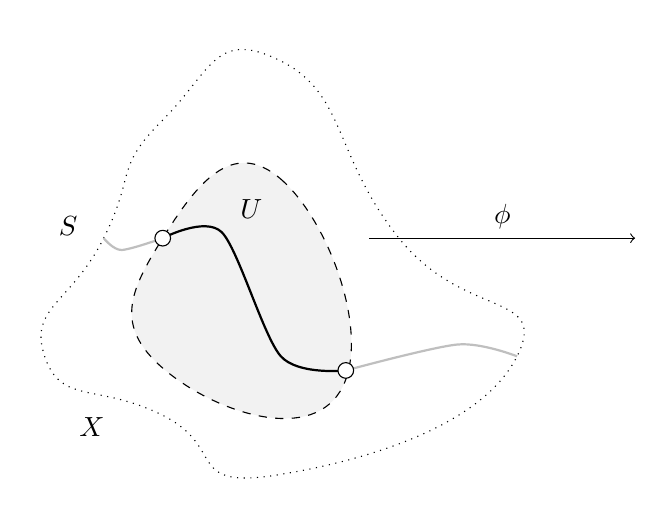
\begin{tikzpicture}[scale=1.5]
	\draw[dotted] plot [smooth cycle, tension=1] coordinates { (0,0) (0.5,1) (1,2) (2,2.5) (3,1) (4,0) (2,-1) (1, -0.5) };
	\draw[dashed,fill=gray,fill opacity=0.1] plot [smooth cycle, tension=1] coordinates { (1,1) (2,1.5) (2.5,-0.3) (1, -0.1) };
	
	
	\draw[thick, lightgray, solid] plot [smooth] coordinates {(0.5,1) (0.65,0.9) (1,1)};
	\draw[thick, black, solid] plot [smooth] coordinates {(1,1) (1.5,1.05) (2,0) (2.55,-0.12)};
	\draw[thick, lightgray, solid] plot [smooth] coordinates {(2.55,-0.12) (3.5,0.1) (4,0)};
	\node[color=white,draw=black,circle,fill,inner sep=2pt] at (1,1) {}; 
	\node[color=white,draw=black,circle,fill,inner sep=2pt] at (2.55,-0.12) {}; 
	
	\node at (0.4,-0.6) {$X$};
	\node at (0.2,1.1) {$S$};
	\node at (1.75,1.25) {$U$};
	\draw[black,->] (2.75,1) -- node[above] {$\phi$} (5,1);
	\end{tikzpicture}
	\begin{tikzpicture}
	\begin{axis}[
	xmin=-1.5,xmax=1.5,
	ymin=-1.5,ymax=1.5,
	ytick={0},
	xtick={0},
	axis lines=middle,
	axis line style=lightgray,
	width=0.5\textwidth,
	axis equal
	] 
	
	
	\addplot[black,dashed] expression[name path=a,domain=-1:1.15,samples=200]{sqrt(1-x^2)};
	\addplot[black,dashed] expression[name path=b,domain=-1:1.15,samples=200]{-sqrt(1-x^2)};
	
	\addplot[fill=gray, fill opacity=0.1]
	fill between[of=a and b,soft clip={domain=-1:1.15}];
	
	\addplot +[mark=none,black,thick,solid,-] coordinates {(-1,0) (1, 0)};
	\node[color=white,draw=black,circle,fill,inner sep=2pt] at (axis cs:-1,0) {}; 
	\node[color=white,draw=black,circle,fill,inner sep=2pt] at (axis cs:1,0) {}; 
	\end{axis}
	\end{tikzpicture}
	\end{center}
	\caption{Suppose $X$ is a manifold (depicted above as an amorphous blob) and $S$ is a subset (depicted above as a squiggly line passing through the blob). Then $S$ is defined to be a \emph{submanifold} of $X$ if $S$ can be covered by charts $(U, \phi)$ such that, under $\phi$, the set $S \cap U$ corresponds to a coordinate hyperplane in $\R^n$. In the picture above, the map $\phi : U \to \R^2$ pulls the squiggle $S \cap U$ taut onto the $x$-axis inside $\R^2$. } \label{submanifold-definition-picture}
\end{figure}

We'll justify the word ``submanifold'' in a moment by showing that submanifolds are actually manifolds in their own right (cf. \cref{submanifolds-are-manifolds}). But first, let's discuss some examples. The intuition you should carry into these examples is roughly that, if a subset ``looks smooth'' (ie, doesn't have any ``pointy'' parts), it should be a submanifold. 

\begin{example}
	Consider the set $S = \{ (x,0) \in \R^2 : -1 < x < 1 \}$ inside $\R^2$. In other words, $S$ is the open interval $(-1,1)$ along the $x$-axis inside $\R^2$. Then $S$ is a submanifold. Indeed, let $U$ be the open box $(-1,1) \times (-1,1)$ inside $\R^2$, and $\phi : U \to \R^2$ the inclusion map. Then $(U, \phi)$ is a chart in the euclidean atlas on $\R^2$, $\phi_2(x,y) = y$, and 
	\[ \{ (x,y) \in U : \phi_2(x, y) = 0 \} = \{ (x,y) \in U : y = 0 \} = S = S \cap U \]
	so $(U,\phi)$ is adapted to $S$ and $S$ has dimension 1 in $(U,\phi)$. 
\end{example}

\begin{example}
	Consider the parabola \[ S = \{ (x, y) \in \R^2 : y = x^2, x \in \R \}. \] This ``looks smooth,'' so it should be a submanifold. Let's see how. It is sufficient to produce a chart $(\R^2, \phi)$ with the property that 
	\[ S = \{ (x,y) \in \R^2 : \phi_2(x,y) = 0 \}. \]
	This means we should take $\phi_2(x,y) = x^2 - y$. Then $\phi_1$ should be a smooth function $\phi_1 : \R^2 \to \R$ such that $\phi = (\phi_1, \phi_2)$ is injective and \'etale. In other words, we want the Jacobian matrix 
	\[ \phi'(x,y) = \begin{bmatrix} \dfrac{\partial \phi_1}{\partial x} & \dfrac{\partial \phi_1}{\partial y} \\ 2x & -1 \end{bmatrix} \]
	to always be invertible. The easiest way to guarantee this is to take $\phi_2(x,y) = x$, which makes $\det \phi'(x,y) = 1$. Moreover, the function $\phi(x,y) = (x, x^2 - y)$ is injective, since if $\phi(x_1, y_1) = \phi(x_2,y_2)$, then $(x_1, x_1^2 - y_1) = (x_2, x_2^2 - y_2)$, and looking at the first coordinates shows that $x_1 = x_2$, and finally looking at the first coordinates shows that $y_1 = y_2$. In other words, $(\R^2, \phi)$ is a slice chart for $S$ in the euclidean atlas, so $S$ is a submanifold of $\R^2$. 
\end{example}

\begin{comment}
	The subset  
	\[ S = \{(x,y) : y = |x|, x \in \R \} \]
	is ``pointy'' and does \emph{not} define a submanifold of $\R^2$. To see this formally, suppose there exists a chart $(U, \phi)$ on $\R^2$ that is adapted to $S$ and contains the origin. By making $U$ smaller, we can assume that $U$ is a box of the form $(-\epsilon, \epsilon) \times (-\epsilon, \epsilon)$. Then $S \cap U$ is neither all of $U$ nor just a point, so it must be that $S$ has codimension 1 in $(U, \phi)$. In other words, 
	\[ S \cap U = \{ (x,y) : \phi_1(x,y) = 0 \}. \]
\end{comment}

\begin{exercise}
	Show that each of the following is a submanifold of $\R^2$. 
	\begin{enumerate}[(a)] 
		\item The $y$-axis. 
		\item The open interval $(-1,1)$ along the $x$-axis.
		\item The line $y = x$.  
		\item The curve $y = x^3$. 
	\end{enumerate}
\end{exercise}

\begin{exercise} \label{circle-submanifold}
	Show that the unit circle $S^1$ is a submanifold of $\R^2$. 
	\begin{hint}
		Let $U = \{(x,y) \in S^1 : x > 0 \}$ and let $\phi(x,y) = (x,x^2+y^2-1)$. See \cref{circle-submanifold-picture}. Show that $(U, \phi)$ is a chart that is adapted to $S^1$. But this one chart does not cover the circle, so then find more charts like this one that cover the circle. 
	\end{hint}
	\begin{figure}
		\begin{center}
			\begin{tikzpicture}
			\begin{axis}[
			xmin=-1.5,xmax=1.5,
			ymin=-1.5,ymax=1.5,
			ytick={0},
			xtick={0},
			yticklabels={},
			axis lines=middle,
			axis line style=lightgray,
			width=0.5\textwidth,
			axis equal
			] 
			
			
			\addplot[white] expression[name path=c,domain=-2:2,samples=2]{1.5};
			\addplot[white] expression[name path=d,domain=-2:2,samples=2]{0};
			\addplot[fill=gray, fill opacity=0.1]
			fill between[of=c and d,soft clip={domain=-2:2}];
			
			\addplot[black,thick] expression[domain=-1:1,samples=200]{sqrt(1-x^2)};
			\addplot[lightgray,thick] expression[domain=-1:1,samples=200]{-sqrt(1-x^2)};
			
			\addplot +[mark=none,black,dashed,->] coordinates {(-2, 0) (1.75, 0)};
			
			\node[color=white,draw=black,circle,fill,inner sep=2pt] at (axis cs:-1,0) {}; 
			\node[color=white,draw=black,circle,fill,inner sep=2pt] at (axis cs:1,0) {}; 
			
			\end{axis}
			\end{tikzpicture}\hspace{1cm}
			\begin{tikzpicture}
			\begin{axis}[
			xmin=-1.5,xmax=1.5,
			ymin=-1.5,ymax=1.5,
			ytick={0},
			xtick={0},
			axis lines=middle,
			axis line style=lightgray,
			width=0.5\textwidth,
			axis equal
			] 
			
			
			\addplot[black,dashed,->] expression[name path=b,domain=-1.575:1.575,samples=200]{x^2-1};
			\addplot[white] expression[name path=a,domain=-1.575:1.575,samples=2]{1.575^2-1};
			\addplot[fill=gray, fill opacity=0.1]
			fill between[of=a and b,soft clip={domain=-2:2}];
			
			\addplot +[mark=none,black,thick,solid,-] coordinates {(-1, 0) (1, 0)};
			
			\node[color=white,draw=black,circle,fill,inner sep=2pt] at (axis cs:-1,0) {}; 
			\node[color=white,draw=black,circle,fill,inner sep=2pt] at (axis cs:1,0) {}; 
			\end{axis}
			\end{tikzpicture}
		\end{center}
		\caption{If $U = \{(x,y) : x > 0\}$ is the right half of the plane and $\phi : U \to \R^2$ is given by $\phi(x,y) = (x^2 + y^2 - 1, x)$, then $(U, \phi)$ is a chart on $\R^2$ that transforms the picture on the left into the picture on the right. The vertical axis on the left turns into the parabola on the right. The top half of the circle on the left turns into the horizontal line segment on right. The vertical axis on the left stays remains the vertical axis on the right.}  \label{circle-submanifold-picture}
	\end{figure}
\end{exercise}

\begin{exercise} \label{graphs-smooth-single}
	Show that the graph of a smooth function $f : \R \to \R$ is a submanifold of $\R^2$. 
\end{exercise}

\begin{caution}
	Sometimes, a subspace that is a manifold can fail to be a submanifold. For example, you might notice that we showed in \cref{graphs-continuous} that the graph of a \emph{continuous} function $\R \to \R$ is a subspace of $\R^2$ and is also a manifold; and then we showed in \cref{graphs-smooth-single} that the graph of a \emph{smooth} function $\R \to \R$ is a submanifold of $\R^2$. And indeed, the graphs of continuous-but-not-smooth functions provide examples of subspaces that are manifolds but not submanifolds. 
\end{caution}

\begin{exercise}
	Let $C$ be the cylinder from \cref{cylinder} and let $L$ be the line \[ L = \{ [1/2, y] \in C : y \in \R \}. \] Show that $L$ is a submanifold of $C$. 
\end{exercise}

We now make good on our promise of proving that submanifolds are in fact manifolds. The proof is a little long because there are a lot of details to check, but there are no real tricks or surprises. 

\begin{proposition} \label{submanifolds-are-manifolds}
	Let $S$ be a submanifold of a manifold $X$. Suppose $(U, \phi) \in \mathscr{A}_X$ is adapted to $S$ and $S$ has dimension $k$ in $(U, \phi)$. Let $\phi|_S : S \cap U \to \R^k$ be the function defined by 
	\[ \phi|_S(p) = (\phi_1(p), \dotsc, \phi_k(p)). \]
	Regarding $S$ as a topological space using the subspace topology, the pair $(S \cap U, \phi|_S)$ is a chart on $S$, and the set of all charts of this form is an atlas on $S$. Thus $S$ becomes a manifold if we equip it with the corresponding maximal atlas $\mathscr{A}_S$. Finally, for any $x \in S$, if $(U, \phi) \in \mathscr{A}_X$ is a slice chart for $S$ containing $x$ such that $S$ has dimension $k$ in $(U,\phi)$, then $\dim_x(S) = k$. 
\end{proposition}

\begin{proof}
	Observe that, by definition, $\phi|_S$ is the composite
	\[ \begin{tikzcd}
	S \cap U \ar[hookrightarrow]{r} & U \ar{r}{\phi} & \R^n \ar{r}{\pi} & \R^{k}
	\end{tikzcd} \]
	where the first map is the inclusion, and the final map $\pi : \R^n \to \R^{k}$ projects onto the first $k$ coordinates (ie, $\pi(x_1, \dotsc, x_n) = (x_{1}, \dotsc, x_k)$). Each of these maps is continuous, so the composite $x|_S$ is continuous as well. The proof that $\phi|_S$ is injective is left as an exercise (cf. \cref{submanifolds-are-manifolds-details}). 
	
	Let us show that $\phi|_S$ is open. By definition of the subspace topology \ref{subspace-topology}, every open subset of $S \cap U$ is of the form $S \cap V$ where $V$ is an open subset of $U$. Suppose $a \in  S \cap V$. We want to show that $\phi|_S(a)$ is an interior point of $\phi|_S(S \cap V)$. Since $V$ is open in $U$ and $\phi : U \to \R^n$ is an open map, we know that $\phi(a)$ is an interior point of $\phi(V)$, ie, there exists $\epsilon > 0$ such that every point of $\R^n$ within $\epsilon$ of $\phi(a)$ is inside $\phi(V)$. We claim that the $\epsilon$ ball around $\phi|_S(a)$ is contained in $\phi|_S(S \cap V)$. In other words, suppose we have $y = (y_{1}, \dotsc, y_k) \in \R^{k}$ such that $|y - \phi|_S(a)| < \epsilon$. We will show that $y \in \phi|_S(S \cap V)$. 
	
	Notice that, since $(U,\phi)$ is a slice chart for $S$, the vector $\phi(a) \in \R^n$ is the same as $\phi|_S(a) \in \R^{k}$ except that for some trailing zeroes. Let $\iota : \R^k \to \R^n$ be the map that concatenates vectors in $\R^{n-k}$ with a string of $n-k$ zeroes. In other words, 
	\[ \iota(y_1, \dotsc, y_k) = (y_1, \dotsc, y_k, \overbrace{0, \dotsc, 0}^{n-k \text{ times}}). \]
	Thus $\phi(a) = \iota(\phi|_S(a))$. Now by the definition of the either the euclidean or the max norm, we see that $|\iota(y) - \phi(a)| = |y - \phi|_S(a)|$, which means that $|\iota(y) - \phi(a)| < \epsilon$. This means that $\iota(y) \in \phi(V)$ due to our choice of $\epsilon$. Since $\phi$ is injective, there exists a unique $b \in V$ such that $\phi(b) = \iota(y)$. This means that the first $k$ coordinates of $b$ are zero, so $b \in S \cap U$ since $(U, \phi)$ is a slice chart for $S$. Moreover
	\[ \phi|_S(b) = \pi(\phi(b)) = \pi(\iota(y)) = y \]
	which shows that $y \in \phi|_S(S \cap V)$. 
	
	Next up, suppose $(U, \phi)$ and $(U', \phi')$ are both charts in $\mathscr{A}_X$ that are adapted to $S$. We want to show that $(S \cap U, \phi|_S)$ and $(S \cap U', \phi'|_S)$ are compatible. If $S \cap U \cap U'$ is empty, there is nothing to do, so we assume that $S \cap U \cap U'$ is nonempty. Let $k$ and $k'$ be the dimensions of $S$ in the two charts $(U, \phi)$ and $(U', \phi')$, respectively. 
	
	The proof of compatibility is encapsulated by the following diagram. 
	\[ \begin{tikzcd}
	\phi|_S(S \cap U \cap U') \ar{r}{(\phi|_S)^{-1}} \ar{d}[swap]{\iota} & S \cap U \cap U' \ar[hookrightarrow]{d} \ar{r}{\phi'|_S} & \phi'|_S(S \cap U \cap U') \\
	\phi(U \cap V) \ar{r}{\phi^{-1}} & U \cap V \ar{r}{\phi} & \phi'(U \cap V) \ar{u}[swap]{\pi'}
	\end{tikzcd} \]
	Here $\iota$ denotes the ``concatenate with $n-k$ trailing zeroes'' map, and $\pi'$ is the ``project onto the first $k'$ coordinates'' map. You should stare at the above diagram until you've convinced yourself that it ``commutes,'' ie, that the result of following any two paths of arrows that start and end at the same place ends up being the same. (The fact that the square on the left of the diagram commutes is because $(U, \phi)$ is a slice chart for $S$, and the fact that square on the right commutes is by definition of the function $\phi'|_S$.)
	
	In other words, the diagram tells us that the transition function $\phi'|_S \circ (\phi|_S)^{-1}$ is equal to $\pi' \circ (\phi' \circ \phi^{-1}) \circ \iota$. Since $(U,\phi)$ and $(U', \phi')$ are compatible, we know that $\phi' \circ \phi^{-1}$ is smooth. Thus the transition function $\phi'|_S \circ (\phi|_S)^{-1}$ is smooth. 
	
	Since $S$ is a submanifold, we know that it can be covered by charts in $X$ that are adapted to $S$. Thus we've just shown that the set
	\[ \mathscr{A} = \{ (S \cap U, \phi|_S) : (U, \phi) \in \mathscr{A}_X \text{ is a slice chart for } S \} \]
	is an atlas on $S$. The assertion about $\dim_x(S)$ follows immediately. 
\end{proof}

\begin{exercise} \label{submanifolds-are-manifolds-details}
	Show that $\phi|_S$ is injective. 
\end{exercise}

\begin{exercise}
	We now have produced two maximal atlases on the unit circle: one we produced in \cref{circle-projection-atlas}, and then another is produced by \cref{circle-submanifold,submanifolds-are-manifolds}. Show that these two maximal atlases are the same. 
\end{exercise}

We've used the word ``submanifold'' once before, in \cref{open-submanifold} where we defined ``open submanifolds.'' Let us now show that this earlier usage of the word ``submanifold'' was justified and does not produce any conflicts with our new definitions.  

\begin{exercise}[``Open submanifolds are submanifolds''] \label{open-submanifolds-are-submanifolds}
	Suppose $X$ is a manifold and $U$ is an open subset. Show that $U$ is a submanifold (in the sense of \cref{submanifold}), and that the maximal atlas on $U$ constructed by \cref{submanifolds-are-manifolds} is equal to the atlas described in \cref{open-submanifold}. 
	\begin{hint}
		Show that a chart $(V, \phi) \in \mathscr{A}_X$ is a slice chart for $U$ if and only if $V \subseteq U$. 
	\end{hint}
\end{exercise}

Here is another property you would hope would be true. 

\begin{exercise}[``Submanifolds of submanifolds are submanifolds'']
	Let $X$ be a manifold, $S$ a submanifold of $X$, and $T$ a submanifold of $S$. Show that $T$ is a submanifold of $X$. 
\end{exercise}

Finally, here is a result that lets us produce many manifolds by considering graphs of smooth functions on euclidean space. 

\begin{proposition} \label{graphs-smooth}
	Suppose $U$ is an open subset of $\R^m$ and $f : U \to \R^n$ is smooth. Then the graph 
	\[ \Gamma = \{ (x,y) \in U \times \R^n : f(x) = y \} \]
	is a submanifold of $U \times \R^n$. 
\end{proposition}

\begin{proof}
	Consider the function $\phi : U \times \R^n \to \R^{m+n}$ given by $\phi(x,y) = (x,f(x)-y)$. Then $\phi$ is injective, since if $\phi(x, y) = (a,b)$, then clearly $x = a$ and $y = f(a)-b$, so any input to $\phi$ is determined by its input. It is also clear that $\phi$ is smooth. If we compute the derivative, we find that  
	\[ \phi'(x,y) = \begin{bmatrix} 
	1 & 0 & \dotsb & 0 & 0 & 0 & \dotsb & 0 \\ 
	0 & 1 & \dotsb & 0 & 0 & 0 & \dotsb & 0 \\
	\vdots & \vdots & \ddots & \vdots & \vdots & \vdots & \ddots & \vdots \\
	0 & 0 & \dotsb & 1 & 0 & 0 & \dotsb & 0 \\ 
	\partial_1 f_1(x) & \partial_2 f_1(x) & \dotsb & \partial_m f_1(x) & -1 & 0 & \dotsb & 0 \\
	\partial_1 f_2(x) & \partial_2 f_2(x) & \dotsb & \partial_m f_2(x) & 0 & -1 & \dotsb & 0 \\
	\vdots & \vdots & \ddots & \vdots & \vdots & \vdots & \ddots & \vdots \\
	\partial_1 f_n(x) & \partial_2 f_n(x) & \dotsb & \partial_m f_n(x) & 0 & 0 & \dotsb & -1
	\end{bmatrix} = \begin{bmatrix} I_n & 0 \\ f'(x) & -I_m \end{bmatrix}, \]
	where $I_r$ denotes the $r \times r$ identity matrix. In other words, the Jacobian matrix $\phi'(x,y)$ is a lower triangular $(n+m)\times(n+m)$ matrix with determinant $(-1)^m$. Thus $\phi$ is \'etale, so $(U \times \R^n, \phi)$ is a chart in the euclidean atlas on $U \times  \R^n$. It is evidently a slice chart for $\Gamma$, proving that $\Gamma$ is a submanifold of $U \times \R^n$. 
\end{proof}

\begin{exercise}
	Suppose $U$ is an open subset of $\R^m$ and $f : U \to \R^n$ is a smooth function. We have discussed two maximal atlases on the graph $\Gamma$ of $f$. One was discussed in \cref{graphs-continuous}, and the other arises by combining \cref{graphs-smooth,submanifolds-are-manifolds}. How do these atlases compare?
\end{exercise}

\subsection{Submersion theorem}

We now have a very important result which let us produce lots of examples of submanifolds of euclidean space out of smooth functions (in the sense of \cref{smooth-multi}). This result goes by many names, including the ``regular level set theorem,'' the ``preimage theorem'' and the ``submersion theorem.'' We will later generalize this result. 

\begin{theorem}[Submersion theorem] \label{submersion-theorem-local}
	Suppose $U$ is an open subset of $\R^m$ and $f : U \to \R^n$ is smooth and submersive. Then $S = f^{-1}(b)$ is a submanifold of $U$ of dimension $m-n$ for any $b \in f(U)$. 
\end{theorem}

\begin{proof}
	By replacing $f$ with the function $x \mapsto f(x)-b$, we can assume without loss of generality that $b = 0$. Fix $a \in S$. We want to find a slice chart for $S$ containing $p$. We know that $f$ is submersive at $a$, which means that the $n \times m$ matrix $f'(a)$ has a non-vanishing $n \times n$ minor. By permuting the coordinates (cf. \cref{permutation-submanifold}), we can assume that it is the $n \times n$ minor on the far right of $f'(a)$ that does not vanish. In other words, we can assume without loss of generality that  
	\begin{equation} \label{derivative-non-vanishing-minor} 
	\det \begin{bmatrix} \partial_{m-n+1} f_1(a) & \dotsb & \partial_{m-n+1} f_1(a) \\ \vdots & \ddots & \vdots \\ \partial_{m} f_n(a) & \dotsb & \partial_{m} f_n(a) \end{bmatrix} \neq 0. 
	\end{equation} Consider the function $\phi : U \to \R^m$ such that, if $x = (x_1, \dotsc, x_m) \in U$, then
	\[ \phi(x) = (x_1, \dotsc, x_{m-n}, f_{1}(x), \dotsc, f_n(x)). \]
	Then 
	\[ \phi'(x) = \begin{bmatrix}
	1 & 0 & \dotsb & 0 & 0 & \dotsb & 0 \\
	0 & 1 & \dotsb & 0 & 0 & \dotsb & 0 \\
	\vdots & \vdots & \ddots & \vdots & \vdots & \ddots & \vdots \\
	0 & 0 & \dotsb & 1 & 0 & \dotsb & 0 \\
	\partial_1 f_{1}(x) & \partial_2 f_{1}(x) & \dotsb & \partial_n f_{1}(x) & \partial_{n+1} f_{1}(x)& \dotsb & \partial_m f_{1}(x) \\ 
	\vdots & \vdots & \ddots & \vdots & \vdots & \ddots & \vdots \\
	\partial_1 f_{n}(x) & \partial_2 f_{n}(x) & \dotsb & \partial_n f_{n}(x) & \partial_{n+1} f_{n}(x)& \dotsb & \partial_m f_{n}(x) \\ 
	\end{bmatrix}. \]
	In other words, the $(m-n) \times (m-n)$ submatrix on the top left is the identity matrix, the $(m-n) \times n$ submatrix on the top right of $\phi'(x)$ is all zeroes, and the bottom $n \times m$ submatrix is precisely $f'(x)$. This means that $\det \phi'(x)$ is equal, up to sign, to the determinant of the $n \times n$ in the bottom right, ie, the $n \times n$ minor on the far right of $f'(x)$. We know from \cref{derivative-non-vanishing-minor} that this minor is nonzero when $x = a$, so $\phi$ is \'etale at $a$. 
	
	Since $f$ is smooth, so is $\phi$, so there exists an open neighborhood $V$ of $a$ such that $\phi|_V$ is \'etale. By the inverse function theorem \ref{inverse-function-theorem}, we can replace $V$ with a smaller open neighborhood of $a$ in order to further assume that $\phi|_V$ is injective. Then \cref{euclidean-chart-characterization} tells us that $(V, \phi)$ is a chart in the euclidean atlas which contains $a$. Moreover, 
	\[ S \cap V = \{ x \in V : f(x) = 0 \} = \{ x \in V : \phi_{m-n+1}(x) = \dotsb = \phi_{m-n+1}(x) = 0 \} \]
	because $\phi_{m-n+j} = f_j$ for all $j = 1, \dotsc, n$. This shows that $(V,\phi)$ is a slice chart for $S$, and that $S$ has dimension $m-n$ at $a$ in $\R^m$. 
\end{proof}

\begin{exercise} \label{permutation-submanifold}
	Suppose $\sigma$ is a permutation of the set $\{1, \dotsc, m\}$. Let $f_\sigma : \R^m \to \R^m$ be the function which ``permutes the coordinates of elements of $\R^m$ according to $\sigma$,'' ie, 
	\[ f_\sigma(x_1, \dotsc, x_m) = (x_{\sigma(1)}, \dotsc, x_{\sigma(m)}). \]
	Show that a subset $S$ is a submanifold of $\R^m$ if and only if $f_\sigma(S)$ is a submanifold of $\R^m$. 
\end{exercise}

\begin{exercise}
	Recall from \cref{circle-projection-atlas,sphere-projection-atlas} that the $n$-sphere $S^n$ is defined by
	\[ S^n = \{ x \in \R^{n+1} : |x|_2 = 1 \}. \]
	Use the submersion theorem to show that $S^n$ is a submanifold of $\R^{n+1}$. 
\end{exercise}

\begin{exercise} \label{torus-equation}
	Let $T$ be the torus inside $\R^3$ centered around the $z$-axis where the distance from the origin to the center of the tube is $R$, the radius of the tube is $r$, and $0 < r < R$. Find a smooth submersive map $f : U \to \R$ where $U$ is an open subset of $\R^3$ and \[ T = \{ (x,y,z) \in U : f(x,y,z) = 0 \}. \]
	Applying the submersion theorem \ref{submersion-theorem-local}, we conclude that $T$ is a submanifold of $\R^3$. 
	\begin{hint}
		See \cref{torus-slice}. 
	\end{hint}
	\begin{figure}[ht]
		\begin{center}
			\begin{tikzpicture}
			\begin{axis}[
			xmin=-4.5,xmax=4.5,
			ymin=-2,ymax=3,
			ytick={0},
			xtick={-3,3},
			xticklabels={$-R$,$R$},
			yticklabels={},
			axis lines=middle,
			axis line style=lightgray,
			width=\textwidth,
			axis equal,
			ylabel={$z$}
			]
			
			\addplot[black,style=thick] expression[domain=2:4,samples=200]{sqrt(1 - (x-3)^2)};
			\addplot[black,style=thick] expression[domain=2:4,samples=200]{-sqrt(1 - (x-3)^2)};
			\addplot[black,style=thick] expression[domain=-4:-2,samples=200]{sqrt(1 - (x+3)^2)};
			\addplot[black,style=thick] expression[domain=-4:-2,samples=200]{-sqrt(1 - (x+3)^2)};
			
			\node[label={45:$(x,y,z)$},color=black,draw=black,circle,fill,inner sep=2pt] at (axis cs:3.5,0.866025) (A) {};
			\node[color=black,draw=black,circle,fill,inner sep=1pt] at (axis cs:3,0) (B) {};
			\node[color=black,draw=black,circle,fill,inner sep=1pt] at (axis cs:3.5,0) (C) {};
			\node[label={$r$}] at (axis cs:3.1,0.3) {};
			
			\draw[black] (B) -- (A) -- (C) -- (B);
			\end{axis}
			\end{tikzpicture}
		\end{center}
		\caption{A slice of the torus $T$ from \cref{torus-equation} along a plane that is perpendicular to the $xy$-plane and contains the $z$-axis.}  \label{torus-slice}
	\end{figure}
\end{exercise}

\section{Smooth functions}

% TODO: Fix notation

We will now define what it means for a function between two manifolds to be smooth. Roughly, the idea is that we know what smooth means on open subsets of $\R^n$, and we just use charts to transfer the definition to arbitrary manifolds. 

Recall that in \cref{multi} we saw that the case when the codomain is $\R$ was the most important. The same will be true here. You may find that the number of definitions of ``smooth'' gets slightly out of hand; if you do, just remember that, whenever multiple definitions of ``smooth'' make sense for the objects in question, they'll all agree. 

\subsection{Smooth real-valued functions}

\subsubsection*{Definition of smoothness for real-valued functions}

\begin{definition}[Smooth real-valued function] \label{smooth-real-valued} \index{smooth}
	Let $X$ be a manifold. A function $f : X \to \R$ is said to be \emph{smooth} if, for any chart $(U, x) \in \mathscr{A}_X$, the function $f \circ x^{-1}$ is smooth.
	\[ \begin{tikzcd} x(U) \ar{r}{x^{-1}} & U \ar{r}{f} & \R \end{tikzcd} \]
\end{definition}

There are two disconcerting things about this definition. First, there is the issue that checking smoothness of a particular function seems next to impossible: the maximal atlas $\mathscr{A}_X$ will have \emph{many, many} charts, some that we may not even know about, and the definition makes it seem like we need to check smoothness on all of them! Thankfully, we don't need to check on all possible charts. As soon as we check smoothness on any atlas, even if it's not maximal, we're done. 

\begin{lemma} \label{smooth-real-valued-local}
	Let $X$ be a manifold and $f : X \to \R$ a function. Suppose that there exists an atlas $\mathscr{A} \subseteq \mathscr{A}_X$ such that $f \circ x^{-1}$ is smooth for any $(U, x) \in \mathscr{A}$. Then $f$ is smooth. 
\end{lemma}

\begin{proof}
	Suppose $(V, y) \in \mathscr{A}_X$. For any $(U, x) \in \mathscr{A}$, we have maps as follows.
	\[ \begin{tikzcd} y(U \cap V) \ar{r}{y^{-1}} \ar{d}[swap]{x \circ y^{-1}} & U \cap V \ar{r}{f} & \R \\ x(U \cap V) \ar[bend right]{ur}[swap]{x^{-1}} \end{tikzcd} \]
	Since $(V, y)$ and $(U, x)$ are both elements of the maximal atlas $\mathscr{A}_X$, we know that the transition function $x \circ y^{-1}$ is smooth. Since $(U, x) \in \mathscr{A}$, we know by assumption that $f \circ x^{-1}$ is smooth. Thus \[ f \circ y^{-1} = (f \circ x^{-1}) \circ (x \circ y^{-1}) \]
	is a smooth function $y(U \cap V) \to \R$. 
	
	Now note that, since $\mathscr{A}$ is an atlas, its charts cover all of $X$, so
	\[ \bigcup_{(U,x) \in \mathscr{A}} y(U \cap V) = y(V). \]
	Since $f \circ y^{-1}$ is smooth when restricted to each the open subset $y(U \cap V)$ for all $(U, x) \in \mathscr{A}$, we conclude that $f \circ y^{-1}$ must be smooth on all of $y(V)$.
\end{proof}

The second disconcerting thing is the following. Suppose $U \subseteq \R^m$ is an open subset and $f : U \to \R$ is a function. On the one hand, we defined what it means for $f$ to be smooth back in \cref{smooth-multi}. On the other hand, we can regard $U$ as an open submanifold of $\R^n$ (cf. \cref{open-submanifold}) and then \cref{smooth-real-valued} gives us another definition of what it means for $f$ to be smooth. A priori, it could be that these definitions conflict. Thankfully, they do not. 

\begin{exercise}
	Suppose $U \subseteq \R^m$ is an open subset and $f : U \to \R$ is a function. Show that $f$ is smooth in the sense of \cref{smooth-multi} if and only if it is smooth in the sense of \cref{smooth-real-valued}. 
	\begin{hint}
		You might find \cref{smooth-real-valued-local} useful. 
	\end{hint}
\end{exercise}

From here on out, we'll use the fact that these two definitions of smoothness coincide without comment. 

\subsubsection*{Combining smooth real-valued functions}

\begin{definition}
	If $X$ is a manifold, we write $\O(X)$ for the set of smooth functions $X \to \R$. 
\end{definition}

Here is the standard set of stability properties we would want. 

\begin{exercise} \label{smooth-real-valued-stable}
	\begin{enumerate}[(a)]
		\item Show that $\O(X)$ is a vector space. 
		\item If $f, g \in \O(X)$, show that $fg \in \O(X)$ also. 
		\item If $f \in \O(X)$ and $f(x) \neq 0$ for all $x$, show that $1/f \in \O(X)$ also. 
		\begin{hint}
			You might decide to do part (d) first, and then use it to prove (c). Or not, you could also just prove (c) directly. 
		\end{hint}
		\item Suppose $f \in \O(X)$, $U$ is an open subset of $\R$, $g : U \to \R$ is smooth, and $f(X) \subseteq U$. Show that $g \circ f \in \O(X)$. 
	\end{enumerate}
\end{exercise}

\begin{unimportantremark}
	if you've taken abstract algebra, you might be interested to notice that the first two stability properties in \cref{smooth-real-valued-stable} show that $\O(X)$ is an $\R$-algebra (ie, that it is simultaneously a commutative ring and a vector space, and that these two structures are ``compatible'' with each other). 
\end{unimportantremark}

\subsubsection*{Smooth approximations of characteristic functions of compact subsets \starred}

Here is a generalization of \cref{constant-compact-zero-outside-neighborhood} which proves, roughly speaking, that we can find a smooth approximation of the characteristic function of a compact subset of a manifold. You may want to look at \cref{compact-topological-space} for the definition of compactness for topological spaces. 

\begin{proposition} \label{smooth-approximation-characteristic-compact}
	Suppose $K$ is a compact subset of a manifold $X$ and $U$ is an open neighborhood of $K$. Then there exists a smooth function $f \in \O(X)$ such that $0 \leq f(x) \leq 1$ for all $x \in \R$, $f(x) = 1$ for all $x \in K$, and $f(x) = 0$ for all $x \notin U$. 
\end{proposition}

\begin{proof}
	Suppose $(V, x)$ is a chart containing some $p \in K$. Recentering, we can assume that $x(p) = 0$ (cf. \cref{recentering-chart}). By shrinking $V$, we can assume that $\bar{V} \subseteq U$ (cf. \cref{smooth-approximation-characteristic-compact-details}). Then $x(V)$ is an open neighborhood of $0 = x(p) \in \R^n$, so there exists $\epsilon > 0$ such that $B(0, \epsilon) \subseteq x(V)$. Let $\psi : \R^n \to \R$ be a bump function supported on $\overline{B}(0, \epsilon)$ (cf. \cref{multivariable-bump-round-support}). Then $\psi \circ x$ is a smooth function on $V$ (cf. \cref{smooth-approximation-characteristic-compact-details}) which is supported entirely inside $V$ (namely, on $x^{-1}(\overline{B}(0,\epsilon))$), and is zero everywhere else on $V$. Define $f_p : X \to \R$ by
	\[ f_p(x) = \begin{cases} \psi \circ x & \text{if } x \in V \\ 0 &  \text{if } x \notin V. \end{cases} \]
	Then $f_p$ is smooth (cf. \cref{smooth-approximation-characteristic-compact-details}), and it is strictly positive on an open neighborhood $V_p$ of $p$ contained inside $U$.  
	
	We can construct such a function $f_p$ for every $p \in K$. Since $K$ is compact, there exist finitely many $p_1, \dotsc, p_n \in K$ such that $K \subseteq V_{p_1} \cup \dotsb \cup V_{p_n}$. Thus $f_{p_1} + \dotsb + f_{p_n}$ is strictly positive on $K$, and zero outside $U$. Since $K$ is compact, there exists $\delta > 0$ such that $f_{p_1} + \dotsb + f_{p_n} \geq \delta$ on $K$ (cf. \cref{smooth-approximation-characteristic-compact-details}). Let $g$ be a bridging function such that $g(x) = 1$ for $x \geq \delta$ and $g(x) = 0$ for $x \leq 0$ (cf. \cref{bridge-function}), and then set $f = g \circ (f_{p_1} + \dotsb + f_{p_n})$.
\end{proof}

\begin{exercise} \label{smooth-approximation-characteristic-compact-details}
	Fill in the missing details in the above proof. 
	\begin{enumerate}[(a)]
		\item Prove that we can ``shrink $V$ in order to assume that $\bar{V} \subseteq U$.''
		\item Modify the bump function of \cref{multivariable-bump-round-support} so that it has support $\overline{B}(0, \epsilon)$. 
		\item Explain why $\psi \circ x$ is a smooth function $V \to \R$. 
		\item Explain why $f_p$ is a smooth function $X \to \R$. 
		\item If $h : K \to \R$ is a continuous function such that $h(x) > 0$ for all $x \in K$, show that there exists $\delta > 0$ such that $h(x) \geq \delta$ for all $x$. 
		
		\begin{hint}
			Let $\delta = \inf\{ h(x) : x \in K \}$ and recall the extreme value theorem. 
		\end{hint}
	\end{enumerate}
\end{exercise}

% TODO: Partitions of unity

\subsection{Smooth functions between manifolds}

Here is a definition that may look a bit terrifying at first. 

\begin{definition}[Smoothness] \label{smooth-between-manifolds} \index{smooth}
	Suppose $X$ and $Y$ are manifolds and $f : X \to Y$ is a function. Then $f$ is \emph{smooth} if, for every chart $(V, y) \in \mathscr{A}_Y$ and every chart $(U, x) \in \mathscr{A}_X$ such that $f(U) \subseteq V$, the function $y \circ f \circ x^{-1} : x(U) \to y(V)$ is smooth. 
	\[ \begin{tikzcd} X \ar{rr}{f} && Y \\ 
	U \ar{rr}{f} \ar[hookrightarrow]{u} \ar{d}[swap]{x} &&  V \ar[hookrightarrow]{u} \ar{d}{y} \\ 
	x(U) \ar{rr}{y \circ f \circ x^{-1}} \ar[hookrightarrow]{d} && y(V) \ar[hookrightarrow]{d} \\ 
	\R^m && \R^n \end{tikzcd} \]
\end{definition}

Once again, we don't need to check all possible charts. The statement is a bit complicated, but it's exactly the statement you might hope for.  

\begin{exercise} \label{smooth-local}
	Suppose $X$ and $Y$ are manifolds and $f : X \to Y$ is a function. Suppose further that there exists an atlas $\mathscr{A} \subseteq \mathscr{A}_Y$ such that, for every $(V, y) \in \mathscr{A}$, there exists an atlas $\mathscr{A}' \subseteq \mathscr{A}_{f^{-1}(V)}$, such that for every $(U, x) \in \mathscr{A}'$, the function $y \circ f \circ x^{-1} : x(U) \to y(V)$ is smooth. Show that $f$ is smooth.
\end{exercise}

We should also note that we haven't redefined the word ``smooth'' in any conflicting ways. More precisely, we have the following two exercises. 

\begin{exercise}
	If $U \subseteq \R^m$ is an open subset and $f : U \to \R^n$ is a function, show that $f$ is smooth in the sense of \cref{smooth-multi} if and only if it is smooth in the sense of \cref{smooth-between-manifolds}.
\end{exercise}

\begin{exercise}
	Show that a function $f : X \to \R$ is smooth in the sense of \cref{smooth-real-valued} if and only if it is smooth in the sense of \cref{smooth-between-manifolds}.
\end{exercise}

From here on out, we'll use the fact that all of these definitions of smoothness coincide without comment. 

Here is an important example of a smooth function. 

\begin{exercise} \label{universal-cover-circle}
	Let $f : \R \to S^1$ be the function $f(t) = (\cos(t), \sin(t))$. Show that $f$ is smooth. 
\end{exercise}

% TODO: Pictures of the universal cover of the circle

\subsubsection*{Combining smooth maps}

It doesn't make sense to add or multiply maps that take values in a manifold. The only thing that makes sense is composition, and indeed, we can compose. 

\begin{exercise} \label{smooth-stable-composite}
	Suppose $X, Y, Z$ are all manifolds and $f : X \to Y$ and $g : Y \to Z$ are smooth. Show that $g \circ f$ is also smooth. 
\end{exercise}  

\subsubsection*{Reduction to smooth real-valued functions}

Finally, we show that the case when the codomain is $\R$ is the most important case. We do this in two steps. 

\begin{proposition} \label{euclidean-valued-smooth-iff-components-smooth}
	Suppose $X$ is a manifold and $f : X \to \R^n$ is a function. Then $f$ is smooth if and only if the component functions $f_i = \pi_i \circ f$ are smooth for all $i = 1, \dotsc, n$. 
\end{proposition}

\begin{proof}
	The single chart $(\R^n, \id)$ is a sub-atlas of the euclidean atlas on $\R^n$, so \cref{smooth-local} says that $f$ is smooth if and only if, for every $(U, x) \in \mathscr{A}_X$, the composite $f \circ x^{-1} : x(U) \to \R^n$ is smooth. This is a function from an open subset of euclidean space into euclidean space, so we know from the definition of smoothness in \cref{multi} that $f \circ x^{-1}$ is smooth if and only if its component functions $\pi_i \circ (f \circ x^{-1})$ are smooth for all $i$. But 
	\[ \pi_i \circ (f \circ x^{-1}) = (\pi_i \circ f) \circ x^{-1} = f_i \circ x^{-1}, \]
	and $f_i \circ x^{-1}$ is smooth for all $(U, x) \in \mathscr{A}_X$ if and only if $f_i$ is smooth, again by \cref{smooth-local}. 
\end{proof}

\begin{proposition} \label{smooth-iff-real-valued-pullbacks-smooth}
	Suppose $f : X \to Y$ is a function between two manifolds. Then the following are equivalent. 
	\begin{enumerate}[(a)]
		\item $f$ is smooth. 
		\item For every open subset $V \subseteq Y$ and every smooth function $g :  V \to \R$, the composite $g \circ f|_{f^{-1}(V)}$ is a smooth function $f^{-1}(V) \to \R$. 
	\end{enumerate}
\end{proposition}

\begin{proof}
	One direction follows immediately from \cref{smooth-stable-composite}. Conversely, suppose $f$ has the property described in (b). Choose a chart $(V, y) \in \mathscr{A}_Y$ of dimension $n$. By assumption, $y_i \circ f|_{f^{-1}(V)}$ is a smooth function $f^{-1}(V) \to \R$ for all $i = 1, \dotsc, n$. By \cref{euclidean-valued-smooth-iff-components-smooth}, this means that $y \circ f|_{f^{-1}(V)}$ is smooth. Since this is true for all charts $(V, y) \in \mathscr{A}_Y$, we conclude that $f$ is smooth.  
\end{proof}

\begin{unimportantremark}
	Suppose $f : X \to Y$ is a smooth function between manifolds. For any $g \in \O(Y)$, we have $g \circ f \in \O(X)$. Thus $g \mapsto g \circ f$ defines a function $f^\sharp : \O(Y) \to \O(X)$, which is actually a homomorphism of $\R$-algebras.
\end{unimportantremark}

\subsection{Paths}

{\color{blue} Incomplete. Gist: we can do basically all we did in \cref{paths-multi} on manifolds, too.}

% TODO: Paths

\subsection{Diffeomorphisms}

Diffeomorphisms are how we formalize the idea that two manifolds are ``basically the same.''

\begin{definition}[Diffeomorphism] \index{diffeomorphism}
	Suppose $X$ and $Y$ are manifolds. A function $f : X \to Y$ is a \emph{diffeomorphism} if it is smooth, bijective, and the inverse function $f^{-1} : Y \to X$ is also smooth. If there exists a diffeomorphism $f : X \to Y$, then $X$ and $Y$ are \emph{diffeomorphic}. 
\end{definition}

\begin{exercise}
	Regard $\R$ as a manifold in two different ways: once with the euclidean atlas, and next with the maximal atlas containing $(\R, x \mapsto x^3)$. Show that these two manifolds are diffeomorphic. 
\end{exercise}

\begin{exercise}
	If $X$ is a manifold and $(U, x) \in \mathscr{A}_X$, prove that $x : U \to x(U)$ is a diffeomorphism. 
\end{exercise}

\begin{definition}[Local diffeomorphism] \index{local diffeomorphism|see {diffeomorphism, local diffeomorphism}} \index{diffeomorphism!local diffeomorphism}
	Suppose $X$ and $Y$ are manifolds. A function $f : X \to Y$ is a \emph{local diffeomorphism} if, for every $p \in X$, there exists an open neighborhood $U$ of $p$ such that $f(U)$ is an open subset of $Y$ and $f|_U$ is a diffeomorphism $U \to f(U)$. 
\end{definition}

\begin{exercise} \label{universal-cover-circle-local-diffeomorphism}
	Consider the smooth function $f : \R \to S^1$ given by $f(t) = (\cos(t), \sin(t))$ from \cref{universal-cover-circle}. Show that $f$ is a local diffeomorphism. 
\end{exercise}

\begin{exercise}
	Show that local diffeomorphisms are smooth and open. 
\end{exercise}